\chapter[Olaf's Fight with Havard]{
    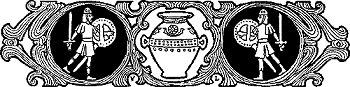
\includegraphics[width=9.3cm]{viking-tales/018}\\
    Olaf's Fight with Havard}

\lettrine{A}{t} another time Harald said:
\vskip2\baselineskip
``Tell me of a fight, Olaf. I want to hear about the music of swords.''

Olaf's eyes blazed.

``I will tell you of our fight with King Havard,'' he said.

``One dark night we had landed at a farm. We left our `Waverunner' in the
water with three men to guard her. The rest of us went into the house.
The farmer met us at the door, but he died by Thorkel's sword. The
others we shut into their beds.\footnote{See note about beds on
page~\pageref{beds}.} The door at each end of the hall we had barred on
the inside so that nobody could surprise us. We were busy going through
the cupboards and shouting at our good luck. But suddenly we heard a
shout outside:

`\,``Thor and Havard!'

``Then there was a great beating at the doors.

`\,``He has two hundred fighters with him,' said Grim; `for we saw his
ships last night. Thirty against two hundred! We shall all drink in
Valhalla to-night.'

`\,``Well,' I cried, `Odin shall have no unwilling guest in me.'

`\,``Nor in me,' cried Hakon.

`\,``Nor in me,' shouted Thorkel.

``And that shout went all around, and we drew out our swords and caught
up our shields.

`\,``Hot work is ahead of us,' said Hakon. `Besides, we must leave none of
this mead for Havard. Lend a hand, some one.'

``Then he and another pulled out a great tub that sat on the floor of the
cupboard.

`\,``I drink to Valhalla to-night,' cried Thorkel the Thirsty, and he
plunged his horn deep into the tub.

``When he brought it up, his sleeve was dripping and the sweet mead was
running over from the horn.

`\,``Sloven!' cried Hakon, and he struck Thorkel with his fist and knocked
him over into the cupboard.

``He fell against the wooden wall at the back, and a carved panel swung
open behind him. He dropped down head first. In a minute he put his head
out of the hole again. We all stood staring.

`\,``I think it is a secret passage,' he said.

`\,``We will try it,' I answered in a whisper. `Throw dirt on the fire. It
must be dark.'

``So we dug up dirt from the earth floor and smothered the fire. All this
time there was a terrible shouting and hammering at the doors, but they
were of heavy logs and stood.

`\,``I with four more will guard this door,' I said, pointing to the east
end.

``Immediately four men stepped to my side.

`\,``And I will guard the other,' Hakon said, and four went with him.

`\,``The rest of you, down the hole!' I said. `Close the door after you. If
luck is with us we will meet at the ships. Now Thor and our good swords
help us! Quick! The doors are giving way.'

``So we ten men stood at the doors and held back the king's soldiers. It
was dark in the room, and the people out of doors could not tell how
many were inside. Few were eager to be the first in.

`\,``Thirty swords are waiting in there to eat up the first man,' we heard
some one say.

``We chuckled at that.

``But the king stood in the very doorway and fought. Our five swords held
him back for a long time, but at last he pushed in, and his men poured
after him. We ran back and hid behind some tubs in a dark corner. The
king's men went groping about and calling, but they did not find us. The
room was full of shouting and running and sword-clashing; for in the
dark and the noise the men could not tell their own soldiers. More than
one fell by his friend's sword. When it was less crowded about the
doorway, I whispered:

`\,``Follow me in double line. We will make for the ships. Keep close
together.'

``So that double line of men, with swords swinging from both sides, ran
out through the dark. Swords struck out at us, and we struck back. Men
ran after us shouting, but our legs were as good as theirs. But I and
Hakon and one other were all that reached the ship. There we saw our
`Waverunner' with sail up and bow pointing to open sea. We swam out to
her and climbed aboard. Then the men swung the sail to the wind, and we
moved off. Even as we went, a spear whizzed through the air, and Hakon
fell dead; for the king and all his men were running to the shore.

`\,``After them!' they were shouting.

``Then we heard the king call to the men in his boats lying out in the
water:

`\,``Row to shore and take us in.'

``Thorkel was standing by my side. At that he laughed and said:

`\,``They do not answer. He left but a handful to guard his ships. They
tasted our swords. And we went aboard and broke the oars and threw the
sails into the water. It will be slow going for Havard to-night.'

\begin{figure}[ht]
    \centering
    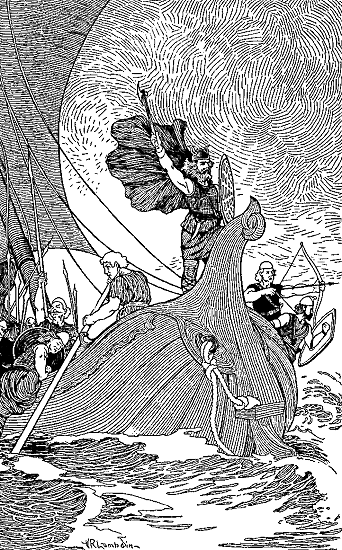
\includegraphics[width=9.1cm]{viking-tales/019}
    \caption{``Then he turned to the shore and sang out loudly''}
\end{figure}

``Then he turned to the shore and sang out loudly:

\begin{quote}
`\,``King Havard's ships are dead:\\
Olaf's dragon flies.\\
King Havard stamps the shore:\\
Olaf skims the waves.\\
King Havard shakes his fist.\\
Olaf turns and laughs.'
\end{quote}

``That was the end of our meeting with King Havard.''

\begin{figure}[hb]
    \centering
    \vskip8pt
    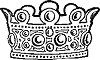
\includegraphics[width=2.7cm]{viking-tales/014}
\end{figure}
